
%(BEGIN_QUESTION)
% Copyright 2014, Tony R. Kuphaldt, released under the Creative Commons Attribution License (v 1.0)
% This means you may do almost anything with this work of mine, so long as you give me proper credit

Identifiser hvilke av disse komponentene som er direkte seriekoblet med hverandre, og hvilke som er direkte parallellkoblet med hverandre:

$$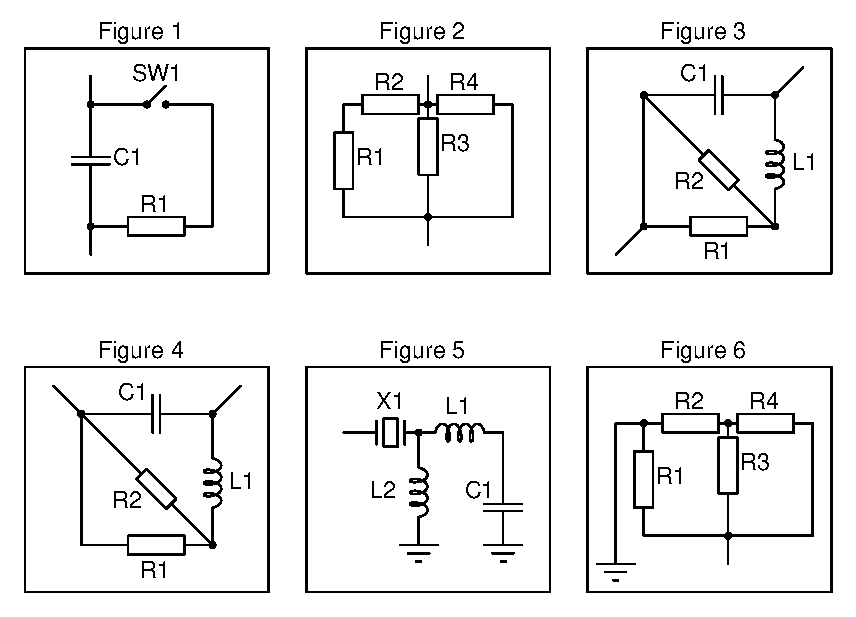
\includegraphics[width=15.5cm]{i01164x01.eps}$$

Anta at de åpne ledningsendene er tilkoblingspunkter til en strømkilde.  I kretser der jordsymbol vises, skal jord regnes som den andre siden av strømkilden.  

\underbar{file i01164}
%(END_QUESTION)





%(BEGIN_ANSWER)

\noindent
{\bf Figur 1:}

R1 seriekoblet med SW1.

\vskip 10pt

\noindent
{\bf Figur 2:}

R1 seriekoblet med R2; R3 parallell med R4.

\vskip 10pt

\noindent
{\bf Figur 3:}

R1 parallell med R2.

\vskip 10pt

\noindent
{\bf Figur 4:}

R1 parallell med R2.

\vskip 10pt

\noindent
{\bf Figur 5:}

L1 seriekoblet med C1.

\vskip 10pt

\noindent
{\bf Figur 6:}

R3 parallell med R4.

%(END_ANSWER)





%(BEGIN_NOTES)

Arbeid sammen med elevene for å tydeliggjøre reglene for hvordan serie- og parallellkoblinger kan identifiseres.  Dette er svært viktig for at elevene skal lykkes med analyse av serie-parallellnettverk.  De vanligste problemene jeg møter som elektronikklærer på dette området, skyldes nesten alltid at elevene ikke konsekvent klarer å skille mellom seriedelnett og parallell-delnett i kombinasjonskretser.

%INDEX% Elektronikkrepetisjon: serie-parallellkretser

%(END_NOTES)

